\documentclass{easychair}

\usepackage{paralist}
\usepackage{xcolor}
\usepackage{amsmath} 
\usepackage{hyperref}
\usepackage{graphicx}
\usepackage{subcaption}
\usepackage{booktabs}
\usepackage{siunitx}
\usepackage{pgfplotstable}
\usepackage{tabularx}
\usepackage{tikz}
\usepackage{xspace}

\DeclareMathOperator*{\argmax}{arg\,max}
\DeclareMathOperator*{\argmin}{arg\,min}

\newcommand{\relu}{\text{ReLU}\xspace{}}

\newcommand{\sat}{\texttt{SAT}}
\newcommand{\unsat}{\texttt{UNSAT}}

\newtheorem{definition}{Definition}


\sisetup{
  round-mode          = places, 
  round-precision     = 7, 
}
   
\hypersetup{
    colorlinks=true,
    linkcolor=magenta,
    urlcolor=blue,
    breaklinks,
    citecolor=blue
}

\pgfplotstableset{
  multistyler/.style 2 args={
    @multistyler/.style={display columns/##1/.append style={#2}},
    @multistyler/.list={#1}
  }
}


\newcommand{\bracketR}[1]{\left(#1\right)}
\newcommand{\bracketS}[1]{\left(#1\right)}
\newcommand{\bracketC}[1]{\left(#1\right)}
\newcommand{\innerproduct}[1]{\left<#1\right>}
\newcommand\norm[1]{\left\lVert#1\right\rVert}


\newcommand{\guy}[1]{\marginpar{\textcolor{orange}{Guy: #1}}}
\newcommand{\ben}[1]{\marginpar{\textcolor{blue}{Ben: #1}}}

\begin{document}

\title{Verifying the Resilience of Neural Network Watermarking}
\author{
Ben Goldberger\inst{1} \and
Yossi Adi\inst{2} \and
Joseph Keshet\inst{2} \and
Guy Katz\inst{1}
}
\institute{
The Hebrew University of Jerusalem, Israel \\
  \{jjgold, guykatz\}@cs.huji.ac.il
  \and
  Bar Ilan University, Israel \\
  yossiadidrum@gmail.com, jkeshet@cs.biu.ac.il
}
\authorrunning{Goldberger, Adi, Keshet and Katz}
\titlerunning{Verifying the Resilience of Neural Network Watermarking}

\maketitle

%% Length: 15 pages

\begin{abstract}
   Add abstract here.
 \end{abstract}

\section{Introduction}
\label{sec:introduction}

\guy{Should we make the title more general? E.g., something like
  ``Minimal Modifications of Deep Neural Networks using Verification''}


\emph{Deep Neural Networks} (\emph{DNN}) are quickly becoming the
state of the art in many domains in computer science.  In fields such
as computer vision, speech recognition, AI, and many others, DNNs
repeatedly demonstrate excellent performance, often matching or even
surpassing other solutions.  As a result of their empiric success,
DNNs are changing the way software is being designed, and are rapidly
being adopted by users in academia and industry.

Along with the increasing pervasiveness of DNNs, there is a growing
need for techniques to (\emph{train}) them efficiently. Unfortunately,
training modern DNNs is far from trivial, often requiring certain
expertise, as well as considerable computing resources. The increasing
demand for specifically designed DNNs has thus given rise to a
\emph{Machine Learning as a Service} (\emph{MLaaS}) paradigm, where
almost-fully-trained DNNs are released by vendors, and clients can
then fine-tune these DNNs to their own needs. This paradigm lets users
enjoy the best of both worlds --- an effective, DNN-based solution,
that can be created using a more reasonable amount of resources.

The MLaaS paradigm holds great potential, but raises two issues that
must be addressed: \emph{authentication of ownership}, and
\emph{minimality of changes}.

\medskip\noindent
\textbf{Authentication of Ownership.}
When vendors allow clients access to an almost-fully-trained network,
they are typically interested in collecting fees and royalties from
each client. This business model compensates the vendor for designing
and training the network, which are not simple tasks. In order to
accomplish this, vendors now seek to imprint their DNNs with
\emph{watermarks}; i.e., to train the DNN in a specific way, such that
when presented with secret, specific inputs the DNN will react in an
unexpected way. Watermarking networks thus gives vendors a way to
recognize, and then claim ownership, over the networks they had
trained.

DNN watermarking holds promise, but raises a concern: if users are
expected to make modifications to the DNN in order to adjust it to
their needs, could they (accidentally or intentionally) remove the
watermarks? In order to address this concern, we require techniques
for generating \emph{resilient watermarks}, i.e. watermarks that are
difficult to remove without damaging the functionality of the DNN in
question.

\medskip\noindent \textbf{Minimality of Changes.}
Modifying an already-trained DNN is a complex task. Typically, a user
would wish to maintain most of the DNN's existing behavior, while
making a small change to its behavior for certain inputs. This task is
an integral part of the MLaaS paradigm, but also arises naturally in
other situations --- e.g., when a bug is discovered in an
already-deployed DNN.

We propose a novel approach for addressing both of these issues, based
on \emph{neural network verification}. DNN verification is an emerging
field, aimed at proving DNN correctness; and existing techniques allow
users to specify properties that involve the DNN's inputs and outputs,
and either prove that these properties hold or provide a
counter-example. Here, we show how to cast the question of making
changes to the DNN itself into the verification setting. We
demonstrate how our new technique can be applied to formally and
accurately measure the resilience of DNN watermarks, and hence to
measure the usefulness of DNN watermarking schemes. We also show how
our technique can be used to identify minimal changes to DNNs, e.g. in
the context of correcting their behaviors for certain inputs. The use
of verification in these contexts guarantees the soundness of our
approach.

For evaluation purposes, we created a proof-of-concept implementation
of our approach as a Python framework. As its underlying backends, our
tool uses the Marabou DNN verification
engine~\cite{KaHuIbJuLaLiShThWuZeDiKoBa19Marabou}, and the Gurobi LP
solver~\cite{gurobi}. We then used our tool to measure the resilience
of a recently-proposed watermarking
scheme~\cite{AdBaPiKeWatermarking}, and also to correct faulty
behavior of DNNs for an airborne collision avoidance
system~\cite{JuLoBrOwKo16,KaBaDiJuKo17Reluplex}. Our results clearly
indicate the usefulness of our approach to real-world examples.

The rest of this paper is organized as follows. In
Section~\ref{sec:background} we provide the necessary background on
DNN's, watermarking, and DNN verification. Next, in
Section~\ref{sec:verifyWatermarks} we introduce our technique for
casting the watermark resilience problem into a verification
problem. Section~\ref{sec:evaluation} describes our implementation and
evaluation of the approach on several watermarked DNN's for image
recognition. We discuss related work in Section~\ref{sec:relatedWork},
and conclude in Section~\ref{sec:conclusion}.

\section{Background}
\label{sec:background}

\subsection{Neural Networks}
A deep neural network is comprised of an input layer, an output layer,
and multiple hidden layers in between. Each layer consists of multiple
nodes (also called neurons), each of which is connected to nodes from
the preceding layer. Each edge that connects two neurons is assigned a
predetermined weight (see Fig.~\ref{fig:dnnExample}). Weight selection
is performed during the DNN's training phase, which is beyond our
scope here --- see, e.g.,~\cite{FoBeCu16}. 


\begin{figure}[htp]
\centering
\scalebox{0.7}{
\def\layersep{2.5cm}
\begin{tikzpicture}[shorten >=1pt,->,draw=black!50, node distance=\layersep]
    \tikzstyle{every pin edge}=[<-,shorten <=1pt]
    \tikzstyle{neuron}=[circle,fill=black!25,minimum size=17pt,inner sep=0pt]
    \tikzstyle{neuron node}=[neuron, fill=blue!50];
    \tikzstyle{annot} = [text width=4em, text centered]

    % Draw the input layer nodes
    \foreach \name / \y in {1,...,4}
        \node[neuron node, pin=left:Input \#\y] (I-\name) at (0,-\y) {};

    % Draw the hidden layer a nodes
    \foreach \name / \y in {1,...,5}
        \path[yshift=0.5cm]
            node[neuron node] (Ha-\name) at (\layersep,-\y) {};
	
	% Draw the hidden layer b nodes
    \foreach \name / \y in {1,...,5}
        \path[yshift=0.5cm]
            node[neuron node] (Hb-\name) at (2*\layersep,-\y) {};

	% Draw the output layer nodes
    \foreach \name / \y in {1,...,3}
        \path[yshift=0.5cm]
        	node[neuron node, pin={[pin edge={->}]right:Output \#\y}] (O-\name) at (3*\layersep,-\y-1) {};    
    % Connect every node in the input layer with every node in the
    % hidden layer.
    \foreach \source in {1,...,4}
        \foreach \dest in {1,...,5}
            \path (I-\source) edge (Ha-\dest);
    % Connect every node in the hidden layer a with the hidden layer b
    \foreach \source in {1,...,5}
        \foreach \dest in {1,...,5}
            \path (Ha-\source) edge (Hb-\dest);
	% Connect every node in the hidden layer b with the output layer
    \foreach \source in {1,...,5}
        \foreach \dest in {1,...,3}
            \path (Hb-\source) edge (O-\dest);

    % Annotate the layers
    \node[annot,above of=Ha-1, node distance=1cm] (hla) {Hidden layer \#1};
    \node[annot,above of=Hb-1, node distance=1cm] (hlb) {Hidden layer \#2};
    \node[annot,left of=hla] {Input layer};
    \node[annot,right of=hlb] {Output layer};
\end{tikzpicture}
}
\caption{An example of a simple deep neural network. The network has
  an input layer of size $4$, two hidden layers of size $5$ each, and an
  output layer of size $3$. The edge weights are omitted.}
\label{fig:dnnExample}
\end{figure}

The neural network is evaluated by assigning values to the input
nodes, and then iteratively propagating these values through the
network, computing the values of additional layers one at a
time. Eventually, the values of the output layer are computed, and
these constitute the network's output.  The value of each hidden node
in the network is computed by calculating a weighted sum of node
values from the previous layers, and then applying a non-linear
\emph{activation function}~\cite{FoBeCu16}.  For simplicity, we focus
here on the Rectified Linear Unit (ReLU) activation
function~\cite{NaHi10} (although our technique is directly applicable
to additional functions as well).  When the ReLU activation function,
$\relu{}(x) = \max{}(0, x)$, is applied to a node, its value is
computed as the maximum between $0$ and the weighted sum computed from
the previous layer.

More formally, let $N$ denote a DNN. we
denote the number of layers in $N$ by $n$, and $s_i$ use to denote the
dimension of layer $i$ (i.e., the number of neurons that it contains).
Layer $1$ is the input layer, layer $n$ is the output layer, and
layers $2,\ldots,n-1$ are the hidden layers.
We use $v_{i,j}$  to denote the value of the $j$'th node of layer $i$,
and use $V_i$ to denote the column vector $[v_{i,1},\ldots,v_{i,s_i}]^T$.
When evaluating $N$ we are given $V_1$, and need to compute $V_n$.
This computation 
performed by using the predefined weights and biases to compute the
layer assignments one by one, each time applying the activation
functions (ReLUs, in our case) to each node. Each layer $2\leq i\leq
n$
is associated
with a 
weight matrix $W_i$ of size $s_{i}\times s_{i-1}$, and also a bias vector $B_i$ of size
$s_i$. The entry of $W_i$ at the $j$'th row and $k$'th column, denoted
$W_i[j,k]$, represents the weight assigned to the edge from
neuron $v_{i-1,k}$ to neuron $v_{i,j}$.
Each hidden layer ($2\leq i \leq n-1$) 
is computed as
\[
V_i = \relu{}(W_i  V_{i-1} + B_i),
\]
with the ReLU
function being applied element-wise.
This rule is applied repeatedly for each layer until $V_{n-1}$ is
calculated.
The final, output layer is
computed similarly, but without an activation function:
\[
  V_n = W_i  V_{n-1} + B_n
\]
For simplicity, in the rest of the paper we assume that
the bias vector $B_i$ is always $0$.

DNNs are often used as \emph{classifiers}, assigning to each input a
label from a finite set of possible labels $L=\{l_1,\ldots,l_{s_n}\}$. In this case, each neuron
in the output layer corresponds to one possible label, and the label
whose neuron is assigned the highest value is the label to which the
input is classified. Thus, an input $V_1$ is classified to label $l_i$
if and only if $v_{n,i}>v_{n,j}$ for every $j\neq i$ (draws are
resolved arbitrarily). We sometimes use the alternative phrasing,
\[
  N(V_1) = \argmax_{1\leq i\leq s_n}\{v_{n,i}\}
\]
A small, running example appears in Fig.~\ref{fig:toyExample}.
\guy{TODO: Ben, please add a toy example, also to serve as our running
  example throughout the paper}

\subsection{Neural Network Verification}


Let $N$ denote a neural network $N$, and let $P,Q$ denote predicates
that encodes some constraints DNN's inputs and outputs, respectively.
\emph{DNN verification} is a field that seeks to answer the question:
does there exist an input $x$ to the DNN such that $P(x)$ and
$Q(N(x))$ both hold, where $N(x)$ represents the network's output when
evaluated on input $x$. Typically, $P$ encodes a set of inputs of
interest, whereas $Q$ encodes the \emph{negation} of a desired
property. If the verification query is \unsat{}, i.e. no such input
$x$ exists, then the desired property is said to hold. Otherwise, the
verification tool returns a concrete counter-example $x_0$ for which
the property in question is violated.


Recently there have been multiple tools and approaches suggested for
solving the DNN verification problem: these include Satisfiabiltiy
Modulo Theories (SMT) based
techniques~\cite{KaBaDiJuKo17Reluplex,KaHuIbJuLaLiShThWuZeDiKoBa19Marabou},
approaches based on mixed integer linear
programming~\cite{Ehlers2017,TjXiTe19}, abstract interpretation based
techniques~\cite{GeMiDrTsChVe18}, and many others
(e.g.,~\cite{HuKwWaWu17,NaKaRySaWa17}. The problem is known to be a
difficult one, and has been shown to be NP-complete even when
restricted to simple cases~\cite{KaBaDiJuKo17Reluplex} (networks with piecewise-linear activation
functions, and properties $P$ and $Q$ that are conjunctions of linear constraints).


\section{Minimal DNN Modification as a Verification Problem}
\label{sec:minimizationProblem}

\subsection{Modifying DNNs}

In all DNN verification approaches to date (to the best of our
knowledge), the goal is to verify a fixed DNN. In other words, $N$ is
given, and a particular input $x_0$ is sought that satisfies certain constraints.
The novelty of our approach is in changing this definition, fixing
the input point $x_0$ (or multiple inputs) and searching for a
\emph{different DNN} $N$ such that certain conditions hold.
More formally, we define the problem as follows:

\begin{definition}\textbf{The DNN Modification Problem.}
  Let $N$ denote a DNN, let $X$ denote a set of fixed input points
  $X=\{x_1, \ldots, x_n\}$, and let $Q$ denote a predicate over the
  classifications $N(x_1),\ldots,N(x_n)$ of the points of $X$. The
  \emph{DNN modification problem} is to find a new DNN, $N'$, such that
  $Q(N'(x_1),\ldots,N'(x_n))$ holds, and such that the distance
  between $N$ and $N'$ is at most some $\delta>0$.
\end{definition}

In this definition we did not yet specify how to measure the distance
between $N$ and $N'$. Multiple measures of distance could be used, but for the
motivating problems that we consider (e.g., verifying the resilience
of watermarks, or finding minimal fixes for erroneous inputs), it
makes sense to require that $N$ and $N'$ share the same topology, and
to define the distance between $N$ and $N'$ according to the
difference in these network's weights. We note that a DNN modification
is trivial if the property $Q$ holds for the original network $N$,
i.e. if $Q(N(x_1),\ldots,N(x_n))$ holds; in that case, $N$ is a
feasible solution to the modification problem.

\begin{definition}\textbf{DNN Distance.}
  Let $N^1$ and $N^2$ denote two DNNs with identical topology,
  i.e. the same number of layers ($n^1=n^2$), and the same number of
  neurons in each pair of matching layers ($s_i^1=s_i^2$ for all
  $1\leq i \leq n^1$). We define the $L$-distance between $N^1$ and $N^2$,
  denoted $\norm{N^1-N^2}_L$, as:
  \[
    \norm{N^1-N^2}_L =    \sum_{i=2}^{n^1}\sum_{j=1}^{s_{i}^1}\sum_{k=1}^{s_{i-1}^1}
    \norm{W^1_i[j,k] - W^2_i[j,k]}_L
  \]
\end{definition}
Intuitively, this definition of distance compares the weight matrices
of the two networks, element-wise; it computes the $L$-distance
between each two corresponding edge weights, and then sums up these
distances. 
Fig.~\ref{fig:toyExampleModified} shows how these definitions are applied
to our toy example from Fig.~\ref{fig:toyExample}.
\guy{TODO: Ben, please continue with the same example from the
  previous section}

Finally, we will typically be interested in finding $N'$ that is
closest to $N$. This is formalized as follows:
\begin{definition}\textbf{The DNN Minimal Modification Problem.}
  Let $N$ denote a DNN, let $X$ denote a set of fixed input points
  $X=\{x_1, \ldots, x_n\}$, and let $Q$ denote a predicate over the
  classifications $N(x_1),\ldots,N(x_n)$ of the points of $X$. The
  \emph{DNN minimal modification problem} is to find a new DNN $N'$
  that solves the DNN modification problem (for $N, X$ and $Q$), such that for every other
  $N''$ that solves the modificaiton problem it holds that
  $\norm{N'-N}\leq \norm{N''-N}$.
\end{definition}
We observe that given a decision procedure for solving the modification
problem, solving the minimal modification problem can be performed by
repeatedly invoking that procedure as part of a binary search.

\subsection{Minimal Modifications as DNN Verification}

A straightforward approach for solving the minimal DNN modification
problem is to cast it as an optimization problem, and use an
off-the-shelf optimization tool. Specifically, the goal would be to
minimize $\norm{N^1-N^2}_L$, while maintaining the constraint
$Q(N'(x_1),\ldots, N'(x_n))$. Unfortunately, such an optimization
problem is highly non-convex and high-dimensional, and is hence very
difficult to solve.

We illustrate this issue in Fig.~\ref{fig:optimizeAllLayers}, using
our running example from~\ref{fig:toyExample}.
\guy{TODO: same example from the previous sections}


In order to mitigate this issue, we focus on a restricted version of
the DNN modification problem, in which the changes in weights are
limited to a \emph{single layer}. We argue that under this
restriction, the DNN modification problem reduces into standard DNN
verification problem. The intuition is as follows: let $N$ be a DNN,
and let $W_i$ ($2\leq i\leq n$) be the only weight matrix of $N$ that
we wish to modify. Observe some fixed input point $x\in X$, and let
$V_{i-1}$ denote the evaluation of layer $i-1$ for this $x$. In the
modified network $N'$, layers $1,\ldots,i-1$ will be assigned the same
values as in $N$, i.e, $V_k=V'_k$ for all $1\leq k\leq i-1$. The
changes in assignment begin only in layer $i$, where it holds that
\[
  V_i' = \relu{}(W_i'V'_{i-1}) = \relu{}((W_i+W_\epsilon)V'_{i-1})
\]
where $W_\epsilon$ represents the change in weights. We note that
$W_i$ and $V'_{i-1}$ are fixed; the only variables here are the
entries of $W_\epsilon$. This means that we can construct a new DNN,
denoted $\bar{N}$, whose input neurons are the values of $W_\epsilon$,
followed by a layer that computes $\relu{}((W_i+W_\epsilon)V'_{i-1})$,
and then feeds into layers $i+1,\ldots,n$ of the original network.

We again illustrate this using our running example --- see
Fig.~\ref{fig:changeJustOneLayer}.


Finally, we note that the restricted version of the problem, in which
we only allow changing a single layer of network, is interesting in
its own right. Specifically, it is is sufficiently expressive for...
\guy{TODO: justify why this is interesting}


\section{Applications}

\subsection{Watermark Resilience}
As briefly discussed in Section~\ref{sec:introduction}, there is now a
growing need to imprint DNNs with \emph{watermarks}: secret inputs,
known to the creator of the DNN, on which the DNN produces unexpected
outputs. Watermarks are important for the MLaaS business model, where
a vendor sells a mostly-trained DNN to clients, who then fine-tune
it for their own needs. The key requirement is that even if the
network undergoes some changes, the watermark input will still produce
the original, unexpected output, allowing the vendor to recognize the
DNN.

More formally, given a DNN $N$, a watermark is just an input point $x$
with a specific label $l$. Typically, a network will have a finite set of
watermarks $X$. Creating this set of watermarks is done at time of
training --- see, e.g.,~\cite{AdBaPiKeWatermarking} for details. We
say that a set $X=\{x_1,\ldots,x_n\}$ of watermarks is $\delta$-resilient if for every
DNN $N'$ such that $\norm{N-N'}\leq \delta$, it holds that
$N(x_i)=N'(x_i)$ for all $1\leq i \leq n$. Clearly, a watermarking
scheme that produces watermarks that are more resilient is preferable.

Solving the DNN minimal modification problem can thus serve two
purposes in the context of watermarking:
\begin{inparaenum}[(i)]
  \item given a specific DNN $N$ and a set $X$ of watermarks, it can
    measure the resilience of $X$ (i.e., the maximal amount of changes
    the network can withstand without ``forgetting'' the watermarks);
    and
  \item given multiple schemes for watermarking DNNs, i.e. for
    producing the set $X$, it can compare the effectiveness of the
    schemes by checking the resilience of the resulting watermarks
    (on some set of DNNs).
\end{inparaenum}
  
\subsection{Minimal Repair}
Despite their overall excellent performance, DNN-based systems are as
prone to error as any other system. Specifically, many erroneous
behaviors have been observed in various DNNs, e.g. for image
recognition~\cite{X,Y} and for airborne collision
avoidance~\cite{JuLoBrOwKo16,KaBaDiJuKo17Reluplex}. Once such a bug is
discovered, it is not immediately clear how to correct it. One
approach would be to retrain the network, but this may be expensive
or impossible for some clients. The approach that we propose here is
simply to identify a \emph{minimal} change to the DNN that removes the
undesirable behavior. We argue that it is useful to focus on a minimal
change here, as such a change is less likely to change the behavior of
the network for other inputs, on which its behavior is currently acceptable.

Finding minimal repairs for a DNN $N$ can be cast into our
formulation, as follows. Given a set of erroneous points
$X=\{x_1,\ldots,x_n\}$ and their set of \emph{correct} labels
$l_1,\ldots,l_n$, we seek a new DNN $N'$ such that $N'(x_i)=l_i$ for
all $1\leq i \leq n$, and such that 
 $\norm{N-N'}$ is minimal. 

\section{Evaluation}

In the watermark problem, we typically have a set of inputs $X=\{x_1,
x_2, \ldots, x_k\}$ with certain classifications
$N(x_1),\ldots,N(x_k)$. We are interested in finding the minimal
change to a DNN $N$ that will remove these watermarks, i.e. change the
classification of the points in $X$. We begin by addressing the case
where $X$ contains a single point $x$, and later expend the discussion
to the more general case.

Observe the input $x$, and observe the prefix of the DNN up to layer
$i-1$. This part of the network is not to be changed; and so, we
evaluate these layers for input $x$, obtaining an assignment for layer
$i$. Denote this assignment vector as $v$; then the output of the
original network is $y=Lv$. The output of the changed network,
however, will be $y'=(L+\varepsilon)v$.

We denote the prediction of the original network as 
\[
   	d_x := argmax_{i\in \bracketsS{m}}\bracketsC{y_i}
\]
And the changed network prediction:
\[
   	d'_x := argmax_{i\in \bracketsS{m}}\bracketsC{y'_i}
\]
And we seek a change $\varepsilon$ to the last layer so that the prediction changes, i.e. $d_x\neq d'_x$.

As previously mentioned, we seek a minimal $\varepsilon$ for which the
label of $x$ changes. As a measure of minimality, we adopt two norms
that are commonly used in the DNN community: the $L_\infty$ and $L_1$
norms. Specifically, 
\begin{equation}
\label{eq:normInf}
   		\norm{\varepsilon}_{\infty}=max_{i,j}\bracketsC{\abs{\varepsilon_{i,j}}}
\end{equation}
And
\begin{equation}
\label{eq:normOne}
   		\norm{\varepsilon}_1=\sum_{i,j}\abs{\varepsilon_{i,j}}.
\end{equation}

When the $\ell_\infty$ norm (\ref{eq:normInf}) is in use, the
aforementioned requirements give rise to a linear programming
minimization problem''
\begin{align*}
\label{eq:LP}
    Minimize:\quad & M \\
    Subject\ to:\quad & \forall i,j\quad -M \leq\varepsilon_{i,j}\leq M \\
    & y'=(L+\varepsilon)v \\
    & y'_{d_x} \leq y'_{d'_x} \\
\end{align*}

Where the variables are the entries in $\varepsilon,y'$ and $M$.
For the $\ell_1$ norm (\ref{eq:normOne}), the minimization problem becomes:
\begin{eqnarray*}
\label{eq:NotLP}
    Minimize:\quad & M \\
    Subject\ to:\quad & \forall i,j\quad -M \leq\sum_{i,j}\abs{\varepsilon_{i,j}}\leq M \\
    & y'=(L+\varepsilon)v \\
    & y'_{d_x} \leq y'_{d'_x} \\
\end{eqnarray*}

Where the variables are the entries in $\varepsilon,y'$ and $M$.

        
\subsection{Defining the problem for multiple inputs}
\label{sec:defineProblem2}

Our definition to a single input minimal change $\varepsilon$ to the network last layer $L$ can be extended to more then one input very easily by adding more constraint to the problem.
\\
Given inputs $\bracketsC{x_1,\cdots,x_k}$ and their respective values:
\begin{align*}
\bracketsC{v_1,\cdots,v_k}\quad: & \text{Inputs to the last layer} \\
\bracketsC{d_1,\cdots,d_k}\quad: & \text{Decisions} \\
\intertext{Such that}
\forall 1\leq j\leq k\quad & d_j = argmax_{i\in\bracketsS{m}}\bracketsC{\bracketsR{L v_j}_i}
\intertext{With chosen new desired decisions
$\bracketsC{d'_1,\cdots,d'_k}$ Such that}
\forall 1\leq j\leq k\quad & d'_j \neq d_j
\end{align*}
\\
our minimization problem for the $\ell_\infty$ norm looks like this:
\begin{equation}
\label{eq:LPmany}
\begin{split}
    Minimize:\quad & M \\
    Subject\ to:\quad & \forall i,j\quad -M \leq\varepsilon_{i,j}\leq M\\
    & \forall j\quad y'_j=(L+\varepsilon)v_j \\
    & \forall j\quad \bracketsR{y'_j}_{d_j} \leq \bracketsR{y'_j}_{d'_j}\\
	\intertext{Variables are the entries in $\varepsilon,y'_1,\cdots,y'_k$ and $M$}
\end{split}
\end{equation}
Similarly for the $\ell_1$ norm the minimization problem looks like that:
\begin{equation}
\label{eq:NotLPmany}
\begin{split}
    Minimize:\quad & M \\
    Subject\ to:\quad & \forall i,j\quad -M \leq\sum_{i,j}\abs{\varepsilon_{i,j}}\leq M\\
    & \forall j\quad y'_j=(L+\varepsilon)v_j \\
    & \forall j\quad \bracketsR{y'_j}_{d_j} \leq \bracketsR{y'_j}_{d'_j}\\
	\intertext{Variables are the entries in $\varepsilon,y'_1,\cdots,y'_k$ and $M$}
\end{split}
\end{equation}

\section{Methods}
\label{sec:methods}

\guy{In this section, explain how the stuff from section 3 can be
  applied to watermarks and network corrections}

As seen in the previous section we have in our hands a minimization problem. One minimization is according to $\ell_\infty$ norm and the other is according to $\ell_a$ norm. In this section we'll show how to convert different problems to the type of minimization problem that was described in the previous section \ref{sec:minimizationProblem}
For the $\ell_\infty$ norm when choosing new predictions all the constraint of the minimization problems (\ref{eq:LP}) (\ref{eq:LPmany}) are linear. There for we choose to solve the $\ell_\infty$ problem using a linear programming solver.
On the other hand $\ell_1$ norm minimization problems (\ref{eq:NotLP}) (\ref{eq:NotLPmany}) have non linear constraint so a linear programming solver is not enough. Instead we used a solver that is capable of dealing with piecewise-linear constraints. 

\subsection{Removing watermarks from neural networks}
\label{sec:removeWatermarks}
A watermarked neural network is a neural network that was trained with a set of inputs and their desired outputs such that the network will still function properly on the task it meant to do, and the output of the network on the set of inputs is as desired (The desired output can be irrelevant to the network task). We'll call the set of inputs and outputs the watermarks of the network \cite{AdBaPiKeWatermarking}. These trained networks are called ``Backdoored'' networks \cite{GuDoSi17BadNet}.
Given a trained watermarked network $N$ with a set of $K$ watermarks inputs and outputs $\bracketsC{\bracketsR{x_1,y_1},\cdots,\bracketsR{x_K,y_K}}$, if we want to remove a specific watermark from the network we can define one of the minimization problems that was described in the previous section (\ref{eq:LP}) (\ref{eq:NotLP}) and search which of the possible decisions (Beside the original decision of the watermark) gives the minimal change.
When removing a set of watermarks of a size $K$ we defined those minimization problem (\ref{eq:LPmany}) (\ref{eq:NotLPmany}), when solving for multiple watermarks we didn't check with combination of possible decisions gets the minimal change because the number of combinations of possible decisions is exponential in $K$, so in order to save time we used a simple heuristic to decide which combination of decisions to check for. 

\section{Evaluation}
\label{sec:evaluation}

We tested both approaches on a simple neural network trained on the MNIST data set, the network have one hidden layer with $150$ nodes. The network was watermarked with $100$ images of noise, examples in Figure \ref{fig:noiseExample}.

\begin{figure}
  \centering
  \begin{subfigure}{0.4\linewidth}
    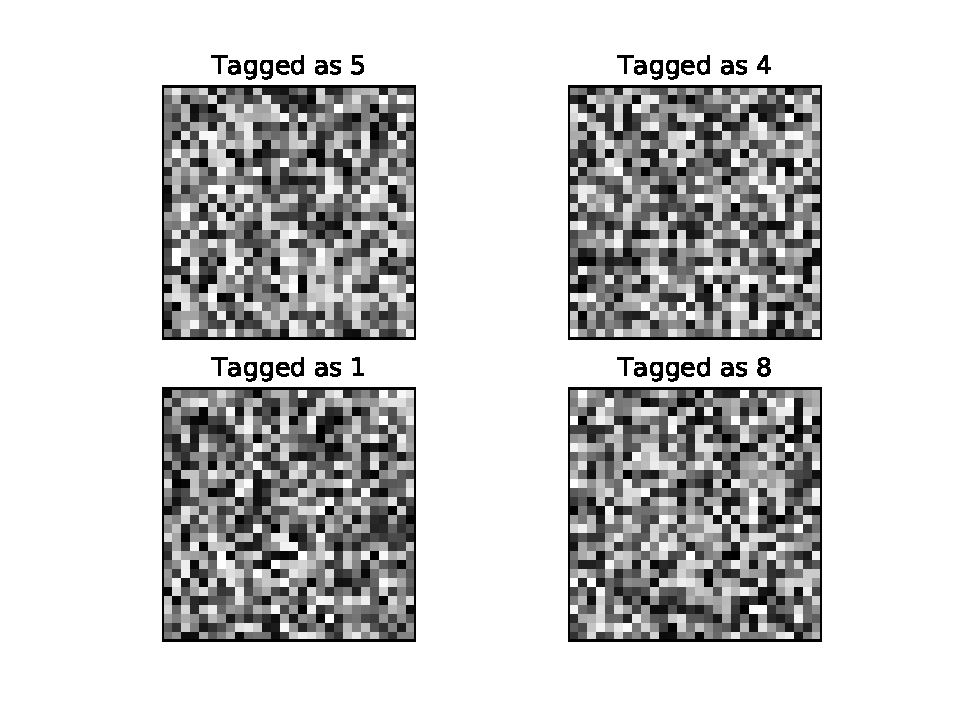
\includegraphics[width=\linewidth]{../data/wm.pdf}
     \caption{Water marks images.}
  \label{fig:noiseExample}
  \end{subfigure}
  \begin{subfigure}{0.4\linewidth}
    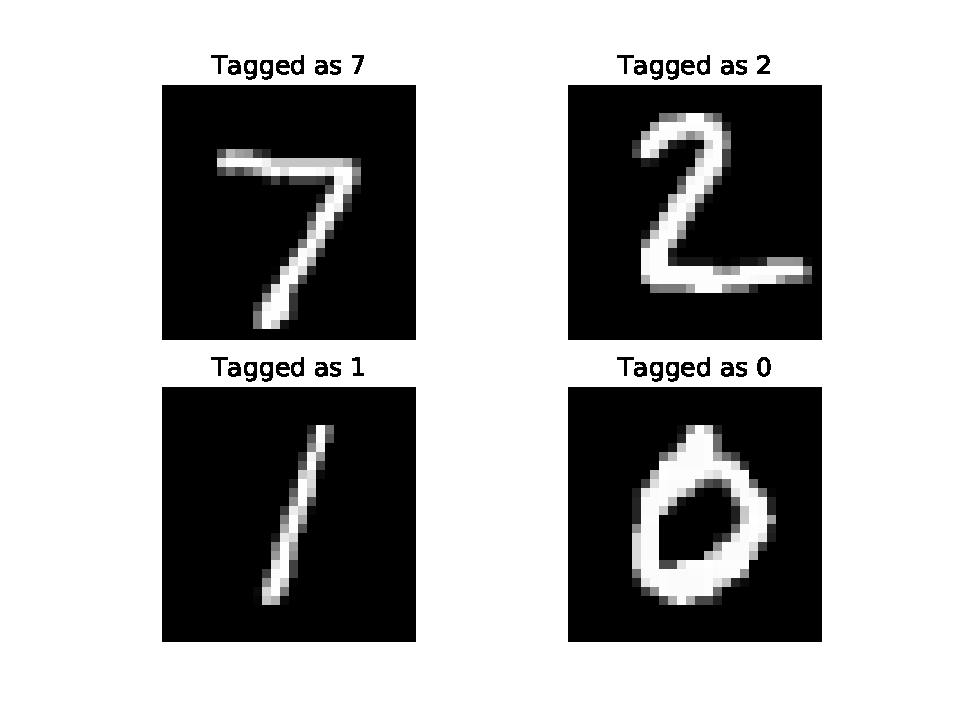
\includegraphics[width=\linewidth]{../data/mnist.pdf}
    \caption{MNIST images.}
  \label{fig:mnistExample}
  \end{subfigure}
\caption{Input images examples.}
\label{fig:inputExample}
\end{figure}

\subsection{Removing a single watermark}
The first test we did was to find the minimal change of a single input as defined \ref{sec:removeWatermarks} for every watermark (noise) image. For every decision possible beside the original decision we found the minimal change and choose the overall minimum. It turns out that the minimal change was always the second best score in the original prediction output. For example an watermark image $w$ with an original output $y$.
\\
\begin{align*}
d_w=&\underset{i\in\bracketsC{0,\cdots,9}}{argmax}\bracketsC{y_i} \\
\intertext{$d_w$ is the original tagging of $w$.}
d'_w=&\underset{i\in\bracketsC{0,\cdots,9}\setminus\bracketsC{d_w}}{argmax}\bracketsC{y_i} \\
\intertext{$d'_w$ will be the new tagging of $w$.}
\end{align*}
\\
So after we apply change to the last layer of the network the new output $y'$ is such that $\underset{i\in\bracketsC{0,\cdots,9}}{argmax}\bracketsC{y'_i}=d'_w$
\\\\
For each watermark image have found the minimal $\varepsilon$. This can give us some measure of how difficult it is to remove a single watermark image. And there may be some correlation in the minimal change distribution that is not related to the norm as seen in this figure \ref{fig:minSingle}. Beside removing a watermark we're interested in the effect the change we introduced have on the network goal. By applying the change to the original network and evaluating on the MNIST dataset we measured the resulting accuracy of each change. As it turns out we get widely different results from both removal methods (norms) when measuring the accuracy of the changed network. As seen in this table \ref{table:singleWatermark} the $\ell_1$ gives better accuracy result on average but can have a bad accuracy result, compered to the $\ell_\infty$ after removing a single watermark that have a consistent result (there minimal accuracy and the maximal accuracy are quite close) but the average is lower then the $\ell_1$ method.
\\\\

\begin{figure}
  \centering
  \begin{subfigure}{0.4\linewidth}
    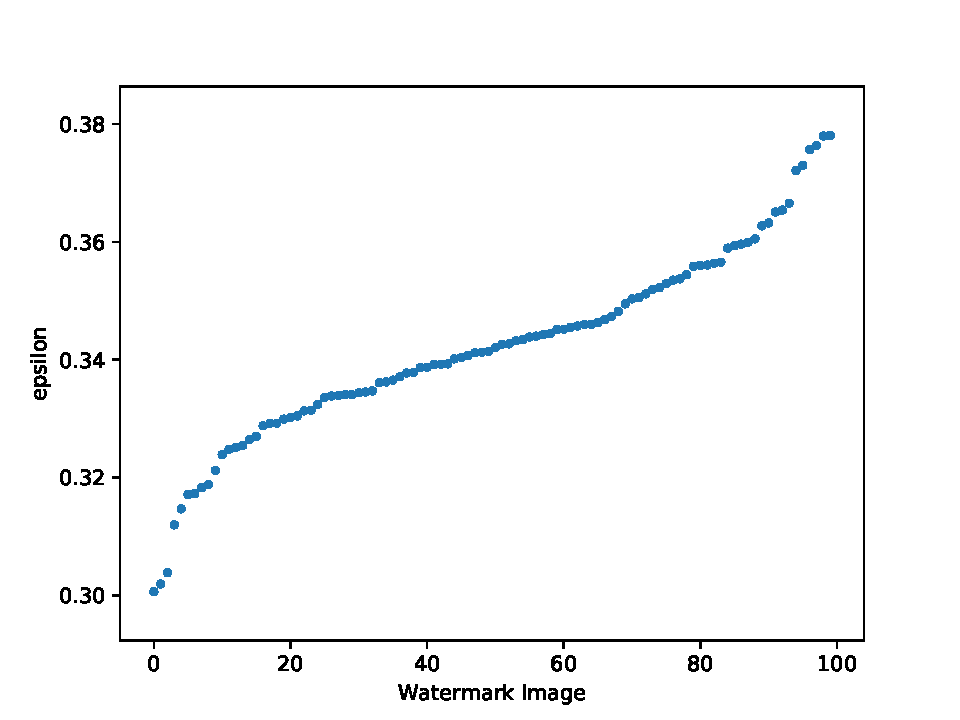
\includegraphics[width=\linewidth]{../data/results/problem3/mnist_w_wm_sorted.pdf}
     \caption{The Minimal $\norm{\varepsilon}_{\infty}$ for every watermark image}
  	\label{fig:minSingleLP}
  \end{subfigure}
  \begin{subfigure}{0.4\linewidth}
    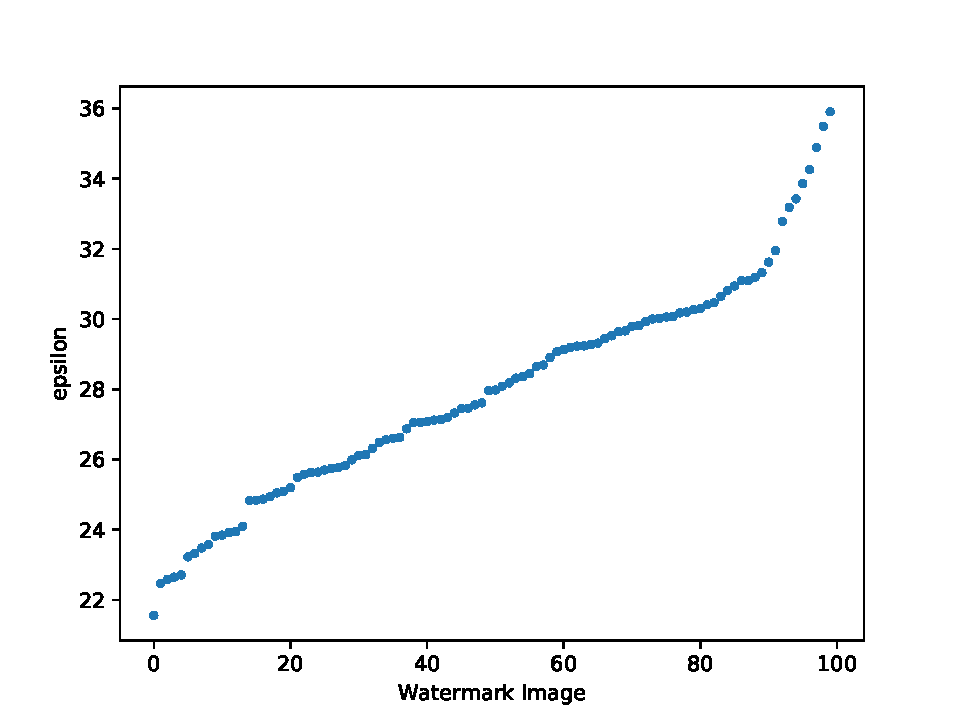
\includegraphics[width=\linewidth]{../data/results/problem2/mnist_w_wm_sorted.pdf}
    \caption{The Minimal $\norm{\varepsilon}_1$ for every watermark image}
  	\label{fig:minSingleNotLP}
  \end{subfigure}
  \caption{Notice the scale of the graphs, the $\ell_\infty$ values are much smaller then the $\ell_1$ values. As expected}
\label{fig:minSingle}
\end{figure}
\begin{table}
\resizebox{\textwidth}{!}{
	\pgfplotstabletypeset[
	every head row/.style={before row=\hline,after row=\hline\hline},
	every last row/.style={after row=\hline},
	col sep=comma,
	columns/Norm/.style={string type},
	every column/.style={column type/.add={|}{}},
	every last column/.style={column type/.add={}{|}}
	]{../data/results/mnist_w_wm_1_wm.csv}
	}
\caption{Minimal changes and Accuracy}
\label{table:singleWatermark}
\end{table}

These results begs the question what is the nature of the change and how it differ between the method? Turns out that when minimizing the change according to $\ell_\infty$ (\ref{eq:LP}) the linear programming solver assign all the entries of $\varepsilon$ a small value. This translate to a change to every weight in the last layer which can explain the uniformity of the accuracy test. On th other hand the when minimizing the change according to $\ell_1$ (\ref{eq:NotLP}) the optimal change is to change only a single entry in $\varepsilon$ by a seemingly large value. So only one weight in the last layer is changed. See figure \ref{fig:lastLayerExampleSingle}
\\
 
\begin{figure}
\centering
  \begin{subfigure}{0.4\linewidth}
  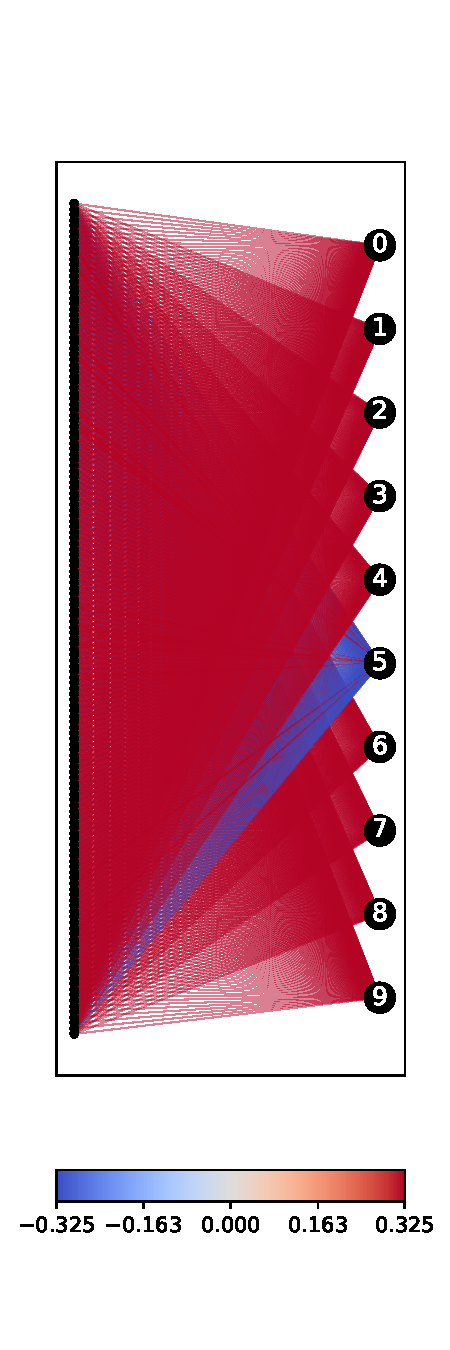
\includegraphics[width=\linewidth]{../data/results/problem3/last_layer_1_wm_example.pdf}
     \caption{The Minimal change according to $\ell_\infty$ for a single input}
  \end{subfigure}
  \begin{subfigure}{0.4\linewidth}
    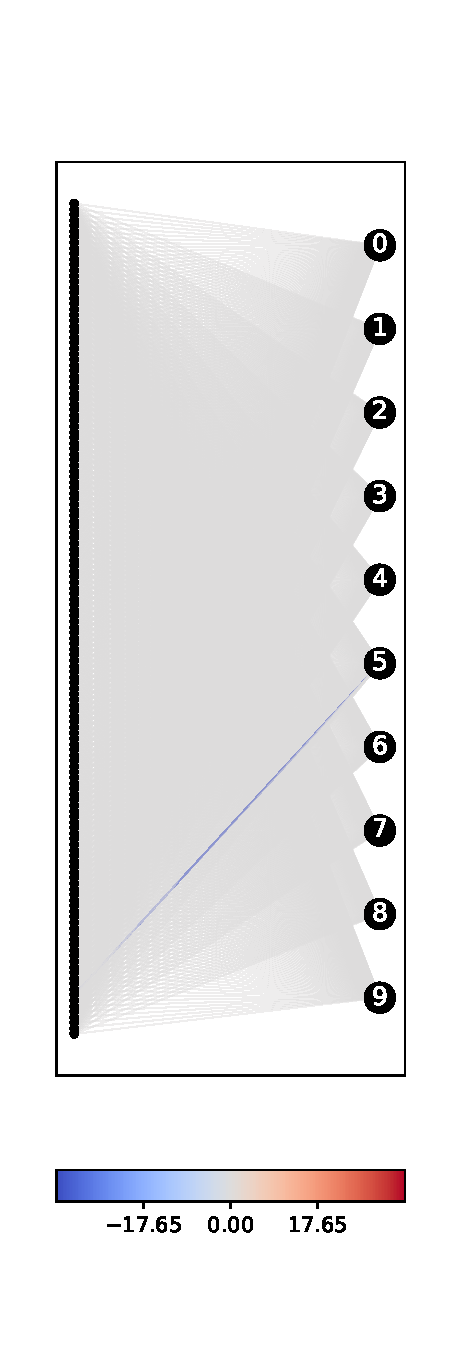
\includegraphics[width=\linewidth]{../data/results/problem2/last_layer_1_wm_example.pdf}
    \caption{The Minimal change according to $\ell_1$ for a single input}
  \end{subfigure}
  \caption{Examples of the change to the last layer. Positive change is colored red and negative change is colored blue. There are $150$ nodes on the left.}
  \label{fig:lastLayerExampleSingle}
\end{figure}

The result of removing a single watermark shows us that the minimal change according to $\ell_\infty$ is changing the network in a broad way and according to the $\ell_1$ norm the change is local, but then not all watermarks are ``equal'', some are harder to remove and some are easy (as seen in the accuracy test \ref{table:singleWatermark}).

\subsection{Removing Multiple watermark}

As described above the removal of watermarks can be generalized to multiple watermarks (\ref{eq:LPmany}) (\ref{eq:NotLPmany}). We tested the same MNIST digits classifying network that is signed with 100 watermark.
\\
While running the problems on multiple watermarks the linear problem that we solved using the Gurobi solver had no issues with scalability and we where able to find the change that fits to as many watermarks as we want, on the other hand the non-linear problem had some issues with scalability so we where able to find the change that fits to up to $5$ watermarks.

\begin{table}
\begin{subtable}{1\textwidth}
\centering
\resizebox{\linewidth}{!}{
	\pgfplotstabletypeset[
	every head row/.style={before row=\hline,after row=\hline\hline},
	every last row/.style={after row=\hline},
	col sep=comma,
	columns/Norm/.style={string type},
	every column/.style={column type/.add={|}{}},
	every last column/.style={column type/.add={}{|}}
	]{../data/results/problem3/mnist_w_wm_summary.csv}
	}
\caption{Change and accuracy when solving for minimal $\ell_\infty$ change.}
\end{subtable}
\begin{subtable}{1\textwidth}
\centering
\resizebox{\linewidth}{!}{
	\pgfplotstabletypeset[
	every head row/.style={before row=\hline,after row=\hline\hline},
	every last row/.style={after row=\hline},
	col sep=comma,
	columns/Norm/.style={string type},
	every column/.style={column type/.add={|}{}},
	every last column/.style={column type/.add={}{|}}
	]{../data/results/problem4/mnist_w_wm_summary.csv}
	}
\caption{Change and accuracy when solving for minimal $\ell_1$ change.}
\end{subtable}
\caption{Minimal changes and Accuracy for multiple watermarks}
\label{table:multipleWatermarks}
\end{table}

\subsection{Network Correction}

We tested our approach to network correction on one of the ACASXU networks and a property that we found bad examples for. We iterated between finding changes to our bad examples and verifying the changed network. Each iteration of our approach is described like that:
\begin{list}{•}{}
\item Given a set of bad examples find the minimal change to the network that will fix those examples. 
\item Verify the changes network.
\begin{list}{•}{}
\item If the verification of the network returns SAT, add the example to our bad examples
\item If the verification of the network returns UNSAT or TIMEOUT and we're finished fixing the network.
\end{list}
\end{list}  

We had two bad example for that network. After finding the minimal change that fixes the erroneous examples we applied that change to the network and verified the network again, that led us to find another erroneous example for the original and changed network. 
We added that erroneous example and find a minimal change to the original network again. After applying that change to the original network the verification of that changed network was timed out.

\begin{figure}
\centering
\begin{subfigure}{0.2\linewidth}
  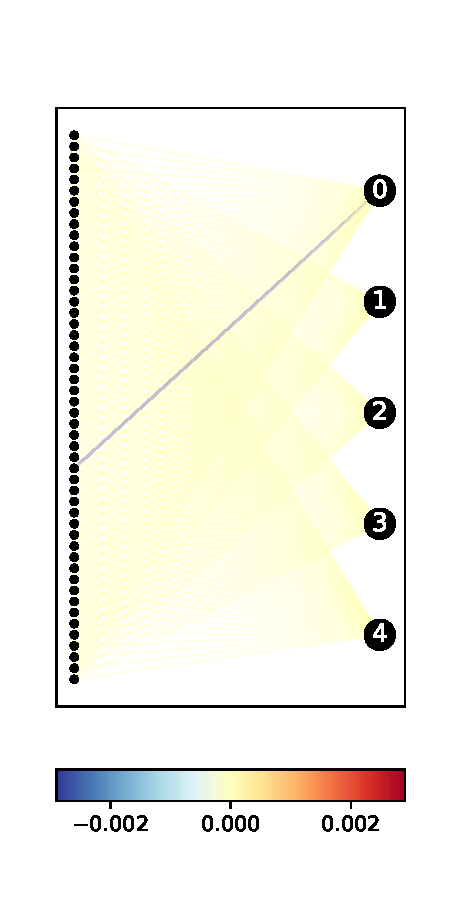
\includegraphics[width=\linewidth]{./images/ACASXU_2_9_1_vals.pdf}
  \caption{First iteration inputs change}
\end{subfigure}
\begin{subfigure}{0.2\linewidth}
  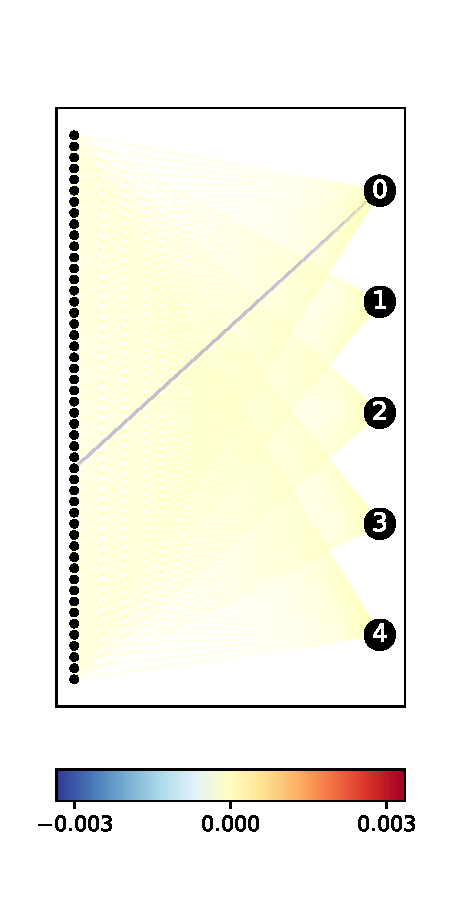
\includegraphics[width=\linewidth]{./images/ACASXU_2_9_3_vals.pdf}
  \caption{Second iteration inputs change}
\end{subfigure}
\caption{Change to the last layer for one of the ACASXU networks.}
\label{fig:lastLayerACASXU}
\end{figure}


\guy{add text about network correction}
\guy{analyze the tables in the text, explain the interesting findings}

\section{Related Work}
\label{sec:relatedWork}

Correcting DNNs in order to remove undesirable behaviors is a general
topic of interest in the ML community. One line of
work~\cite{KaLe18,KaFu18} suggests to augment a malfunctioning DNN
with decision trees that determine when a patch should be
applied. Another line of work~\cite{SoTh19} corrects DNNs using an
iterative encoding of the problem into a sequence of Max-SMT
instances. A key feature of our verification-based approach that
separates it from prior work is that it provides provides formal
guarantees about the minimality of the discovered changes to the DNN
in question.

DNN verification is an emerging field, with many recently-proposed
tools and approaches. These include the use of SMT
solving~\cite{HuKwWaWu17,KaBaDiJuKo17Reluplex,KaHuIbJuLaLiShThWuZeDiKoBa19Marabou},
LP and MILP solving~\cite{Ehlers2017,TjXiTe19}, symbolic interval
propagation~\cite{WaPeWhYaJa18}, abstract
interpretation~\cite{GeMiDrTsChVe18}, and many others
(e.g.,~\cite{BuTuToKoMu18,DuJhSaTi18,LoMa17,NaKaRySaWa17,SiGePuVe19}).
Our technique reduces the DNN minimal modification problem into a DNN
verification problem, and can use many of the aforementioned tools and
techniques as a backend.

DNN watermarking is a general approach for marking DNNs that are to undergo
changes, for which multiple methods have been proposed in recent years~\cite{AdBaPiKeWatermarking,ChRoKo18,LePeTr19,UcNaSaSa17,VeUsTaOcGa11}
Our technique can be applied in order to assess the
performance of watermarking approaches and compare them to each other.


\section{Conclusion and Future Work}
\label{sec:conclusion}

\subsection*{Acknowledgments}
The project was partially supported by grants from the Binational Science
Foundation (2017662) and the Israel Science Foundation (683/18).

\guy{TODO: Ask the Yossis for additional acks}

\bibliographystyle{abbrv}
\bibliography{watermarks}

\end{document}

%%% Local Variables:
%%% mode: latex
%%% TeX-master: t
%%% End:
